\documentclass[11pt]{article}
\usepackage[utf8]{inputenc}
\usepackage[T1]{fontenc}
\usepackage[margin=1in]{geometry}
\usepackage{amsmath,amssymb,amsthm}
\usepackage{booktabs}
\usepackage{array}
\usepackage{url}
\usepackage{microtype}
\usepackage{graphicx}
\usepackage{caption}
\usepackage{xcolor}
\usepackage{listings}
\usepackage[hidelinks]{hyperref}
\makeatletter\g@addto@macro{\UrlBreaks}{\do\_\do\.\do\/}\makeatother
\emergencystretch=3em
\tolerance=2000
% generated by gen_inputs.py; do not edit
\newcommand{\DXNComp}{21}
\newcommand{\DXNQuench}{12}
\newcommand{\DXNAnneal}{2}
\newcommand{\DXNIncomm}{2}
\newcommand{\DXNSqNoise}{5}
\newcommand{\DXNPos}{10}
\newcommand{\DXNAtLattice}{4}
\newcommand{\DXNAbove}{17}
\newcommand{\DXNUndercut}{0}
\newcommand{\DXNOpen}{14}
\newcommand{\DXNDesignedNeg}{7}
\newcommand{\DXQuenchLattice}{3}
\newcommand{\DXQuenchDefected}{7}
\newcommand{\DXAnnealLattice}{1}
\newcommand{\DXMinRelComp}{-2.3\times10^{-14}}
\newcommand{\DXMinRelAll}{-2.6\times10^{-14}}
\newcommand{\DXMaxAbsPos}{2.6\times10^{-14}}
\newcommand{\DXMinAbove}{1.54\times10^{-4}}
\newcommand{\DXMaxSfDiff}{1.6\times10^{-5}}
\newcommand{\DXSqNoiseMin}{1.73\times10^{-3}}
\newcommand{\DXSqNoiseMax}{4.77\times10^{-3}}
\newcommand{\DXSqNegMin}{64}
\newcommand{\DXSqNegMax}{72}
\newcommand{\DXIcEwaldTri}{8.5\times10^{-14}}
\newcommand{\DXIcEwaldSq}{1.9\times10^{-13}}
\newcommand{\DXIcDirect}{1.9\times10^{-5}}
\newcommand{\DXIcNegCtl}{3.14\times10^{-2}}
\newcommand{\DXEtaGrid}{4.8\times10^{-13}}
\newcommand{\DXEtaRefs}{1.3\times10^{-13}}
\newcommand{\DXBoxCell}{2.6\times10^{-14}}
\newcommand{\DXGridN}{41}
\newcommand{\DXGridDmin}{0.01}
\newcommand{\DXGridDmax}{3}
\newcommand{\DXSqRelLo}{1.58\times10^{-2}}
\newcommand{\DXSqRelHi}{1.36\times10^{-3}}
\newcommand{\DXHcRelLo}{9.53\times10^{-2}}
\newcommand{\DXHcRelHi}{8.75\times10^{-3}}
\newcommand{\DXEtriSmallD}{4.4462}
\newcommand{\DXDproxyA}{6.599}
\newcommand{\DXDMoSe}{6.5827}
\newcommand{\DXDWSe}{6.6151}
\newcommand{\DXDMoS}{6.2371}
\newcommand{\DXDtElev}{0.0209}
\newcommand{\DXDtTwelve}{0.0660}
\newcommand{\DXDtThreeTwelve}{0.1143}
\newcommand{\DXTestsPassed}{28}
\newcommand{\DXTestsFailed}{0}
\newcommand{\DXTestsIgnored}{1}
\newcommand{\DXRecompileCtl}{rc 0 in 755.4 s, axiom output identical to stage 1}
\newcommand{\DXRecompileSrc}{rc 0 in 660.7 s, axiom output identical to the stage-1 compile}
\newcommand{\DXShaPrior}{b85389a50373adaf877e866c79f0696ba0a284d9626bc9a56040821c3e11f27d}
\newcommand{\DXShaMulti}{7f52ea64903c43cbfe95b76eea74a2ea01040c45d778ae05bbb848aa9554f98a}
\newcommand{\DXShaCtl}{1754e1a9ba6ed844a1d0356872cf2a5662c89d13e85d1fd39747f3fe1215106d}
\newcommand{\DXShaAnyD}{0a6d86eef3ee24b2b6828ff602707868e160969bfbebc41db375c05b383c5168}
\newcommand{\DXShaMatch}{match}
\newcommand{\DXShaStepOne}{ceb2c607498086e8f865ebeee944842548345501d704a54b0dfc465cd9f42f7d}
\newcommand{\DXShaStepOneCtl}{8a26b6ba14882ad6fc3e57cc69376786c30993695fc50846fc8a75add1ca4987}
\newcommand{\DXShaStepOneMatch}{match}
\newcommand{\DXStepOneBuild}{rc 0 in 22.7 s}
\newcommand{\DXStepOneCtl}{rc 0 in 16.4 s}
\newcommand{\DXLedgerN}{33}
\newcommand{\DXLedgerA}{14}
\newcommand{\DXLedgerL}{4}
\newcommand{\DXLedgerC}{7}
\newcommand{\DXLedgerX}{8}
\newcommand{\DXGateExit}{1}
\newcommand{\DXGateBlock}{0}
\newcommand{\DXGateFlag}{14}
\newcommand{\DXmeVElev}{0.0014}
\newcommand{\DXmeVTwelve}{0.044}
\newcommand{\DXmeVThreeTwelve}{0.223}

\lstset{basicstyle=\ttfamily\footnotesize,columns=fullflexible,keepspaces=true,breaklines=true,
  frame=single,framesep=3pt,xleftmargin=4pt,xrightmargin=4pt,upquote=true,
  keywordstyle=\bfseries,morekeywords={theorem,lemma,def,noncomputable,abbrev,where,fun,Prop,axiom},
  escapeinside={(*@}{@*)}}
\newtheorem{theorem}{Theorem}
\newtheorem{lemma}[theorem]{Lemma}
\theoremstyle{remark}
\newtheorem{remark}[theorem]{Remark}
\newcommand{\R}{\mathbb{R}}
\newcommand{\tier}[1]{\textsf{[#1]}}
\newcommand{\lean}[1]{\texttt{#1}}
\newcommand{\dt}{\tilde d}
\makeatletter\newcommand{\tabinput}[1]{\@@input #1 }\makeatother

\title{The bilayer dipolar-exciton interaction\\ is completely monotone in $r^2$:\\ kernel-checked triangular-lattice
corollaries at every density\\ and an exact-Ewald CVODE consistency study}
\author{Xavier Callens (SocrateAI Lab)}
\date{Preprint v1, 2026-10-25}
\hypersetup{pdftitle={Bilayer dipolar-exciton interaction: kernel-checked triangular-lattice corollaries},
  pdfauthor={Xavier Callens}}

\begin{document}
\maketitle
\begin{center}\small doi:10.5281/zenodo.23646103 \quad (not peer reviewed)\end{center}


\noindent\textbf{AI-assistance disclosure.} This preprint, its Lean code, its Rust and Python code and its claim ledger
were produced by AI agents (Claude, Anthropic) under the author's direction. The author is responsible for the content.
No human has audited the Lean statements for adequacy, and no human referee has checked the hand proofs. A separate AI
agent instance audited this preprint (verdict ACCEPT\_WITH\_CORRECTIONS, no blocking findings); this version applies
its corrections (\texttt{AUDIT.md}, \texttt{REVISION.md}).

\begin{abstract}
Two rigid, vertically aligned electron--hole dipoles in a bilayer, at layer separation $d$ and in-plane distance $r$,
interact by $V(r)=2\bigl(1/r-1/\sqrt{r^2+d^2}\bigr)$ in units of $e^2/(4\pi\varepsilon)$. As a function of $t=r^2$ this
is $g_d(t)=2\bigl(t^{-1/2}-(t+d^2)^{-1/2}\bigr)$.

\textbf{Tier A (Lean~4.34.1, pinned openai/math).} The axiom footprint is $\{$\lean{propext}, \lean{Classical.choice},
\lean{Quot.sound}$\}$, and the planted \lean{sorry} and planted-axiom controls are caught. We prove that $g_d$ is
admissible in upstream's sense (smooth, nonnegative, completely monotone on $(0,\infty)$). The same holds for the whole
family $t^{-s/2}-(t+c)^{-s/2}$ with $s>0$, $c\ge0$; for $c<0$ it fails, a negative control. With upstream's
\lean{universal\_energy\_minimum} this gives triangular-lattice optimality among locally finite configurations at
density one and, through a rescaling theorem, at every density $\rho>0$. For $g_d$ ($d>0$) we also prove that the
optimal energy is finite, at density one and at every density, so those inequalities are not $\top\le\top$; no finiteness
theorem is proved for the rest of the family. The algebraic identity $g_d(r^2)=2(1/r-1/\sqrt{r^2+d^2})$ is
kernel-checked as well. Every optimality statement is \emph{conditional} on that upstream
theorem, which is AI-generated and not peer reviewed (the planar Cohn--Kumar conjecture was stated open in the human
literature in 2019~\cite{ps}), and on the fidelity of its definitions.

\textbf{Tier C.} The physics reading and a step-by-step human proof for undergraduates. Complete monotonicity of $g_d$
is elementary; the only new item is the explicit kernel-checked corollary. We claim no breakthrough.

\textbf{Tier X.} A new rusty-SUNDIALS module computes exact Ewald energies of the untruncated potential. It agrees with an
independent Python Ewald sum to $\le\DXIcEwaldSq$ relative. CVODE gradient-flow relaxations found
\DXNUndercut{} of \DXNComp{} relaxed periodic competitors below the triangular lattice; only \DXNOpen{} of them are open
searches, the other \DXNDesignedNeg{} are designed negative controls. A HuggingFace JARVIS-DFT mirror
supplies a proxy layer spacing $d\approx\DXDproxyA$~\AA{} for MoSe$_2$/WSe$_2$, which places the experimental exciton
densities at $\dt=d\sqrt n\approx0.02$--$0.11$.
\end{abstract}

\paragraph{Tiers.} \tier{A}: kernel-checked Lean, with axioms within the allowlist and planted controls caught.
\tier{L}: a cited source, quoted in the ledger (prose as extracted, mathematics transcribed linearly, elisions
marked). \tier{C}: an argument or human proof that is not
machine-checked. \tier{X}: floating-point exploration, which never supports a claim. Identifiers such as
\texttt{DX-A-0004} refer to \texttt{ledger/ledger.json} (Section~\ref{sec:ledger}). A Tier~A tag attaches to the Lean
statement, never to its physical gloss. Status words: the four prior-round theorems (\texttt{DipolarExciton.lean}) were
recompiled by a separate AI verifier with verdict ACCEPT\_WITH\_CORRECTIONS; the new module
(\texttt{DipolarExcitonMultipolar.lean}) was re-elaborated from source by a separate AI auditor at the stage-4 audit
(rc~0, axioms within the allowlist, the auditor's own planted \lean{sorry} and planted axiom caught); the small
Step-1 module added in this revision (\texttt{DipolarExcitonStep1.lean}) is \emph{producer-checked only}. No module
has had a human audit.

\section{Setting}\label{sec:setting}
Upstream~\cite{oai} calls $g:\R\to\R$ \emph{admissible} if it is $C^\infty$ on $(0,\infty)$, $g\ge0$ there, and
$(-1)^n g^{(n)}\ge0$ for all $n$. The pair interaction of two points $x,y$ in the plane is $g(\|x-y\|^2)$: $g$ is a
function of the \emph{squared} distance. The energy of a configuration $C$ is the $\liminf$ over radii $R$ of the
average, over points in the closed disk of radius $R$, of the sum over all other points in the disk; this is the lower
energy (1.1) of Petrache--Serfaty~\cite{ps} \tier{L, DX-L-0001}. \lean{latticeEnergy} sums $g(\|a\|^2)$ over all nonzero
points of the density-one triangular lattice $A$. Upstream proves that $A$ has the least energy among locally finite
density-one configurations \tier{A, DX-A-0001}; the rescaling theorem D2 of~\cite{d2} extends this to every density
\tier{A, DX-A-0002}. Petrache and Serfaty (2019) state that the planar Cohn--Kumar conjecture ``remains open in
dimension 2'' \tier{L, DX-L-0001}; we did not re-check its status after 2019 for this paper, so DX-A-0001 is an AI-generated claim on an open problem, accepted here only as a kernel-checked
statement about upstream's definitions.

\lstinputlisting[caption={Upstream definitions and theorems (openai/math pinned copy, and D2 \texttt{AnyDensity.lean}; proofs elided).},label=lst:up]{gen/upstream.lst}

\section{Step-by-step human demonstration}\label{sec:human}
This section is for a strong undergraduate. Each step states the fact, proves it, and names the Lean declaration that
checks it. The physics of Step~1 is \tier{C} and its algebra \tier{A}; Steps 2--9 are mirrored in Lean \tier{A}.

\lstinputlisting[caption={The potential, its negative control, and the shifted-difference family (verbatim).},label=lst:defs]{gen/defs.lst}

\paragraph{Step 1: the pair potential \tier{C, DX-C-0001}.} Exciton $i$ is an electron at height $d$ directly above a hole
at height $0$, both at in-plane position $x_i$. For two excitons with $|x_i-x_j|=r$ there are four Coulomb pairs: the two
electrons (distance $r$, $+1/r$), the two holes ($+1/r$), and two electron--hole cross pairs at distance $\sqrt{r^2+d^2}$
(each $-1/\sqrt{r^2+d^2}$). The binding inside each exciton is a constant and is dropped. Hence
$V(r)=2/r-2/\sqrt{r^2+d^2}$, and with $t=r^2$ we get $V(r)=g_d(r^2)$. Since $\sqrt{r^2+d^2}>r$, $V>0$, and at large
$r$, $V(r)=d^2/r^3+O(r^{-5})$, the dipole--dipole law. The pair counting (which charges sit where, the factor~2,
dropping the intra-exciton binding) is the physical reading and stays at Tier~C. The algebra is kernel-checked
\tier{A, DX-A-0013}: $g_d(t)=2(1/\sqrt t-1/\sqrt{t+d^2})$ for $t>0$ (\lean{g\_sqrt}), hence
$g_d(r^2)=2(1/r-1/\sqrt{r^2+d^2})$ for $r>0$ (\lean{g\_inplane}, using $\sqrt{r^2}=r$), and $g_d(r^2)>0$ for $d\ne0$
(\lean{g\_inplane\_pos}); Listing~\ref{lst:step1}. The proof of \lean{g\_sqrt} is the stage-4 auditor's probe, moved
unchanged into a claimed module.

\paragraph{Step 2: derivatives of a shifted power.} For real $a$, $c\ge0$, $t>0$ and $r\in\mathbb N$,
\[\frac{d^r}{dt^r}(t+c)^a=a(a-1)\cdots(a-r+1)\,(t+c)^{a-r}=\mathrm{desc}_r(a)\,(t+c)^{a-r}.\]
\emph{Proof.} Induction on $r$: differentiating $(t+c)^{a-r}$ gives $(a-r)(t+c)^{a-r-1}$, and
$\mathrm{desc}_{r+1}(a)=\mathrm{desc}_r(a)(a-r)$. The base $t+c>0$, so every power is differentiable there. By linearity,
$g_d^{(r)}(t)=2\,\mathrm{desc}_r(-\tfrac12)\bigl(t^{-1/2-r}-(t+d^2)^{-1/2-r}\bigr)$.
Lean: \lean{iteratedDeriv\_rpow}, \lean{iteratedDeriv\_shift}, \lean{iteratedDeriv\_g} (Listing~\ref{lst:steps}).

\paragraph{Step 3: the sign.} $(-1)^r\mathrm{desc}_r(-\tfrac12)=\prod_{k=0}^{r-1}(-1)(-\tfrac12-k)
=\prod_{k=0}^{r-1}(\tfrac12+k)=\mathrm{asc}_r(\tfrac12)>0$, a product of positive numbers. Lean: \lean{sign\_desc}
(Mathlib's \lean{ascPochhammer\_eval\_neg\_eq\_descPochhammer} and \lean{ascPochhammer\_pos}).

\paragraph{Step 4: the bracket.} For $e\le0$ the map $x\mapsto x^e$ is nonincreasing on $(0,\infty)$. With
$e=-\tfrac12-r$ and $t\le t+d^2$ we get $t^{e}-(t+d^2)^{e}\ge0$. Lean: \lean{diff\_nonneg}.

\paragraph{Step 5: admissibility \tier{A, DX-A-0003}.} Steps 2--4 give
$(-1)^r g_d^{(r)}(t)=2\,\mathrm{asc}_r(\tfrac12)\bigl(t^{-1/2-r}-(t+d^2)^{-1/2-r}\bigr)\ge0$; $r=0$ is $g_d\ge0$.
Smoothness: $t\mapsto t^a$ and $t\mapsto(t+c)^a$ are $C^\infty$ where the base is positive. So $g_d$ is admissible.
Replacing $\tfrac12$ by $s/2$ ($s>0$) and $d^2$ by $c\ge0$ changes nothing, which gives \lean{shiftDiff\_admissible}; a
nonnegative multiple of an admissible function is admissible (\lean{admissible\_const\_mul}), and
$g_d=2\,\mathrm{shiftDiff}_{1,d^2}$ (\lean{g\_eq\_shiftDiff}), so $g_d$ is admissible for \emph{every} real $d$
(\lean{dipolar\_admissible\_all}) \tier{A, DX-A-0007}. Statements: Listings~\ref{lst:prior} and~\ref{lst:multi}. (Equivalently, by Bernstein,
$t^{-1/2}-(t+c)^{-1/2}=\pi^{-1/2}\int_0^\infty e^{-ut}(1-e^{-uc})u^{-1/2}\,du$, a positive mixture of exponentials
\tier{C, DX-C-0003}.)

\paragraph{Step 6: triangular optimality at density one \tier{A, DX-A-0004}.} Apply upstream (Listing~\ref{lst:up}) to
$g_d$: for every locally finite density-one $C$, $\mathrm{latticeEnergy}(g_d)\le\mathrm{energy}(g_d,C)$. This step is
exactly as strong as upstream. Lean: \lean{triangular\_dipolar\_optimal}.

\paragraph{Step 7: the bound is not $\top\le\top$ \tier{A, DX-A-0005}.} Put $a=t^{-1/2}$, $b=(t+c)^{-1/2}$, so
$0<b\le a$, $a^2t=1$ and $b^2(t+c)=1$. Then $a^2-b^2=a^2b^2\bigl((t+c)-t\bigr)=c\,a^2b^2$, i.e.
$(a-b)(a+b)=c\,a^2b^2$. Since $b\le a$, $2b^2\le a^2+ab=a(a+b)$, hence $2(a-b)(a+b)\le c\,a^3(a+b)$, and dividing by
$a+b>0$, $a-b\le\tfrac c2\,t^{-3/2}$. With $c=d^2$: $g_d(t)\le d^2t^{-3/2}$. The triangular lattice sum of
$\|a\|^{-3}$ converges (Riesz exponent $3>2$), so $\mathrm{latticeEnergy}(g_d)\le d^2\,\mathrm{latticeEnergy}(t^{-3/2})<\infty$.
Lean: \lean{diff\_le}, \lean{g\_le}, \lean{latticeEnergy\_dipolar\_lt\_top} (with \lean{latticeEnergy\_riesz\_lt\_top}).

\paragraph{Step 8: every density \tier{A, DX-A-0010, DX-A-0011}.} If $C$ has density $\rho$, then $\sqrt\rho\,C$ has density
one, and $\|\sqrt\rho x-\sqrt\rho y\|^2=\rho\|x-y\|^2$, so the $g$-energy of $C$ is the $g(\cdot/\rho)$-energy of
$\sqrt\rho\,C$. The function $t\mapsto g(t/\rho)$ is admissible (each derivative gains the positive factor $\rho^{-r}$).
Upstream applied to $g(\cdot/\rho)$ then says $\rho^{-1/2}A$ is optimal at density $\rho$. This is D2's
\lean{triangular\_optimal\_any\_density}, instantiated as \lean{triangular\_dipolar\_optimal\_any\_density}. Non-vacuity:
$g_d(t/\rho)\le d^2\rho^{3/2}t^{-3/2}$ (\lean{g\_scaled\_le}), so the optimal energy is finite
(\lean{energy\_dipolar\_any\_density\_lt\_top}); statements in Listing~\ref{lst:dens}. Physically, $g_d(t/\rho)=\sqrt\rho\,g_{d\sqrt\rho}(t)$: density $\rho$
at separation $d$ is density one at separation $\dt=d\sqrt\rho$, with energies scaled by $\sqrt\rho$
\tier{C, DX-C-0004}; this identity is not kernel-checked and is not needed by Lean.

\paragraph{Step 9: negative controls \tier{A, DX-A-0006, DX-A-0008}.} (i) $h_d(t)=t^{-1/2}-2(t+d^2)^{-1/2}$ (cross
attraction weighted twice): at $t=d^2$, $h_d=1/d-2(2d^2)^{-1/2}<1/d-2(4d^2)^{-1/2}=0$, so $h_d$ is not admissible
(\lean{h\_neg\_at}, \lean{h\_not\_admissible}). (ii) For $c<0$ and $t=-2c>0$, $t+c=-c\in(0,t)$, so
$(t+c)^{-s/2}>t^{-s/2}$ and $\mathrm{shiftDiff}_{s,c}(t)<0$ (\lean{shiftDiff\_not\_admissible\_of\_neg}). The sign
of the shift is load-bearing, and a gate that accepted these would be broken.

\begin{remark}[scope of non-vacuity]\label{rem:c0}
The finiteness theorems of Steps~7--8 are proved for $g_d$ only. The family corollaries
\lean{triangular\_shiftDiff\_optimal} and \lean{triangular\_shiftDiff\_optimal\_any\_density} \tier{A, DX-A-0009} carry no
finiteness theorem; at $c=0$, $\mathrm{shiftDiff}_{s,0}\equiv0$ and their conclusion is the trivial $0\le\mathrm{energy}$.
\end{remark}

\lstinputlisting[caption={Step lemmas (statements verbatim, proofs elided).},label=lst:steps]{gen/steps.lst}

\section{Lean formalization}\label{sec:lean}
Prior-round module \texttt{formal\_cert/Autoresearch/DipolarExciton.lean} (namespace \lean{AutoresearchDipolar}),
imported unchanged, and the new module \texttt{DipolarExcitonMultipolar.lean} (namespace
\lean{AutoresearchDipolarMultipolar}). Both are compiled with the pinned toolchain (Lean~4.34.1, Mathlib
\texttt{d13f23b7}, openai/math \texttt{fd4aeeb2}). \texttt{grep -c sorry} on both claimed modules gives 0. Planted
controls live only in \texttt{DipolarExcitonMultipolarControls.lean}. At the stage-4 audit a separate AI agent
recompiled both modules from source (\texttt{DipolarExciton.lean} rc~0 in 62.9~s, \texttt{DipolarExcitonMultipolar.lean}
rc~0 in 56.9~s; \texttt{audit/recompile\_*\_src.json}) and caught its own planted \lean{sorry} and planted axiom in a
separate probe file (\texttt{audit/audit\_controls.json}); all 16 re-printed claimed declarations stayed within the
allowlist. This revision adds a third claimed module, \texttt{DipolarExcitonStep1.lean} (namespace
\lean{AutoresearchDipolarStep1}, \DXStepOneBuild; \texttt{grep -c sorry} gives 0), with planted controls in
\texttt{DipolarExcitonStep1Controls.lean} (\DXStepOneCtl): \lean{ctl1\_sorry} is flagged with \lean{sorryAx},
\lean{ctl1\_axiom} with the planted \lean{ctl1\_cheat}, and \lean{ctl1\_wrong\_sign\_false} proves that the wrong-sign
in-plane form fails at $r=d=1$ \tier{A, DX-A-0014}:
\lstinputlisting[basicstyle=\ttfamily\scriptsize]{gen/axioms_step1_controls.txt}

\lstinputlisting[caption={Prior-round theorems (verbatim statements).},label=lst:prior]{gen/prior.lst}
\lstinputlisting[caption={New: the shifted-difference family and its negative control (independently recompiled by an AI auditor; no human audit).},label=lst:multi]{gen/multi.lst}
\lstinputlisting[caption={New: every density and non-vacuity for $g_d$ (independently recompiled by an AI auditor; no human audit).},label=lst:dens]{gen/density.lst}
\lstinputlisting[caption={Revision: the Step-1 identity (producer-checked only).},label=lst:step1]{gen/step1.lst}

\paragraph{Axiom audit and planted controls \tier{A, DX-A-0012}.} The controls file imports the built module, plants
\texttt{theorem ctl\_sorry : (1 : $\mathbb N$) = 2 := sorry} and \texttt{axiom ctl\_cheat : False}, and prints the axioms of
every claimed theorem. Verbatim output (stage~1, \texttt{contribution/compile\_controls.json}):
\lstinputlisting[basicstyle=\ttfamily\scriptsize]{gen/axioms_controls.txt}
The file exits with rc~0 \emph{despite} the planted \lean{sorry} and axiom, so the exit code is not the gate; the axiom
list is. Both controls are flagged (\lean{sorryAx}, \lean{ctl\_cheat}); every claimed theorem is within the allowlist.

\section{Physics: what the theorem does and does not say}\label{sec:phys}
\paragraph{System and units.} Interlayer (indirect) excitons in a transition-metal-dichalcogenide heterobilayer such as
MoSe$_2$/WSe$_2$: electrons in one layer, holes in the other, bound into dipoles of length $\approx d$. Energies are in
units of $e^2/(4\pi\varepsilon_0\varepsilon_r)$ per length; lengths in the numerics are in units of $n^{-1/2}$ (density
one), and $\dt=d\sqrt n$ \tier{C, DX-C-0004}.

\paragraph{What it says \tier{C, DX-C-0002}.} In the classical, zero-temperature model of rigid point dipoles
perpendicular to the layers, with unscreened Coulomb interactions, no locally finite configuration at any fixed density
has lower lower-energy than the triangular lattice, conditional on upstream and on definition fidelity.

\paragraph{What it does not say.} It is not a uniqueness statement (finite perturbations of $A$ have the same
$\liminf$ energy~\cite{ps}). It contains no kinetic or zero-point energy, so it says nothing about quantum (bosonic)
exciton liquids or condensates. It has no dielectric screening (h-BN, Rytova--Keldysh), no moir\'e potential, no
in-plane electron--hole offset, no separate electron and hole crystals, and no electron--hole plasma. Experiments on
h-BN-encapsulated MoSe$_2$/WSe$_2$ at 4~K report moir\'e-trapped excitons below $n\sim1$--$5\times10^{11}$~cm$^{-2}$, a
free exciton gas only ``in the narrow density range around $10^{11}\sim10^{12}$~cm$^{-2}$'', a Mott transition at
$n_\mathrm{Mott}=1.6$--$3\times10^{12}$~cm$^{-2}$, and moir\'e wells ``of the order of 10s-100 meV'' deep~\cite{wang}
\tier{L, DX-L-0002}. In that window real interlayer excitons are a quantum gas, not a classical crystal
\tier{C, DX-C-0007}.

\section{rusty-SUNDIALS numerics}\label{sec:num}
Everything in this section is \tier{X}: it illustrates the Tier~A statement and checks consistency, and supports no
claim. Code: \texttt{crates/qf-yukawa-crystal} (\texttt{dipolar.rs}, \texttt{dipolar\_ewald.rs},
\texttt{bin/dipolar\_crystal.rs}) on branch \texttt{physics/ar-dipolar-exciton-2026-10-25}; the preregistration
(DIP-TRI-1) was committed before the solver code (Section~\ref{sec:repro}).

\paragraph{Method.} The code uses the rescaled form $U=V/\dt^2=2/(r\,s\,(r+s))$, $s=\sqrt{r^2+\dt^2}$, which has no
cancellation at small $\dt$ and tends to $1/r^3$. Exact energies of periodic configurations of the \emph{untruncated}
potential use an Ewald split of $V(r)=\frac{4}{\sqrt\pi}\int_0^\infty e^{-r^2u^2}(1-e^{-\dt^2u^2})\,du$ at $u=\eta$:
real-space part $2(\operatorname{erfc}(\eta r)/r-\operatorname{erfc}(\eta s)/s)$, reciprocal part including $G=0$ (the
potential is integrable, so no background is needed), and self term. The per-particle energy is
$e=\tfrac12\sum'U$, so $\mathrm{latticeEnergy}(g_d)=2d^2e_\mathrm{tri}$ in these units \tier{C, DX-C-0006}. Dynamics
use a shifted-force truncation at $r_c=8$ only to \emph{generate} competitors: overdamped gradient flow integrated with
CVODE (BDF, analytic Jacobian $=-$Hessian, rtol $10^{-10}$, atol $10^{-12}$) until $\max|F|<10^{-9}$, for
$N=288$ particles in a $16a\times9\sqrt3a$ box that holds the triangular lattice exactly. Every reported energy and
gap is the Ewald value. \emph{Deviation from DIP-TRI-1:} the preregistered \texttt{reported\_potential} was the periodic
image sum to radius $R$ plus the analytic uniform tail; we report Ewald energies instead, because that truncated sum
leaves the non-monotone residual described below (Figure~\ref{fig:trunc}).

\paragraph{Correctness controls \tier{X, DX-X-0001}.} An independent Python Ewald sum (adaptive \texttt{scipy} quadrature,
$\eta=1.0$ against $0.8$ in Rust) agrees to $\le\DXIcEwaldTri$ (triangular) and $\le\DXIcEwaldSq$ (square) relative at
the five $\dt$ values. Python direct sums with $R=100$--$400$ plus the exact uniform tail $2\pi n/(\sqrt{R^2+\dt^2}+R)$
agree to $\le\DXIcDirect$, the size of the oscillating lattice-minus-continuum residual. \emph{Negative control:}
dropping the tail gives an error of $\DXIcNegCtl$. The Rust energy is $\eta$-independent to $\le\DXEtaRefs$ (five $\dt$,
$\eta\in\{0.6,0.8,1.2\}$) and $\le\DXEtaGrid$ (\DXGridN-point grid), and the 288-particle box matches the primitive
cell to $\le\DXBoxCell$. As $\dt\to0$, $e_\mathrm{tri}\to\DXEtriSmallD$ at $\dt=\DXGridDmin$, which should be half the
density-one triangular Riesz-3 lattice sum; we did not compare it with a literature value. The stage-4 auditor's
independent check (\texttt{audit/audit\_epstein\_check.py}, no Ewald sum: expansion in $\dt^2/r^2$ and closed-form
Epstein zeta functions, mpmath, with its own positive and negative controls) reproduces $e_\mathrm{tri}$ and
$e_\mathrm{sq}$ at $\dt=0.0209,0.066,0.114,0.3$ to about $10^{-13}$ relative and gives the exact $\dt\to0$ limit
$4.446373$, consistent with the grid value \tier{X, DX-X-0001}. A plain spherical
cutoff with tail leaves a non-monotone residual of up to $1.7\times10^{-3}$ at $R=8$ and $4.0\times10^{-5}$ at $R=64$
(Figure~\ref{fig:trunc}) \tier{X, DX-X-0005}, which is why only Ewald gaps are reported.

\begin{table}[t]\centering\small
\caption{Exact (Ewald) per-particle energies in $U=V/\dt^2$ units and lattice gaps \tier{X, DX-X-0002}.}\label{tab:lat}
\begin{tabular}{rrrrr}\toprule
$\dt$ & $e_\mathrm{tri}$ & $e_\mathrm{sq}-e_\mathrm{tri}$ & $e_\mathrm{hc}-e_\mathrm{tri}$ & $e_\mathrm{sq}/e_\mathrm{tri}-1$\\\midrule
\tabinput{gen/table_lattice.tex}\bottomrule\end{tabular}
\end{table}

\begin{figure}[t]\centering
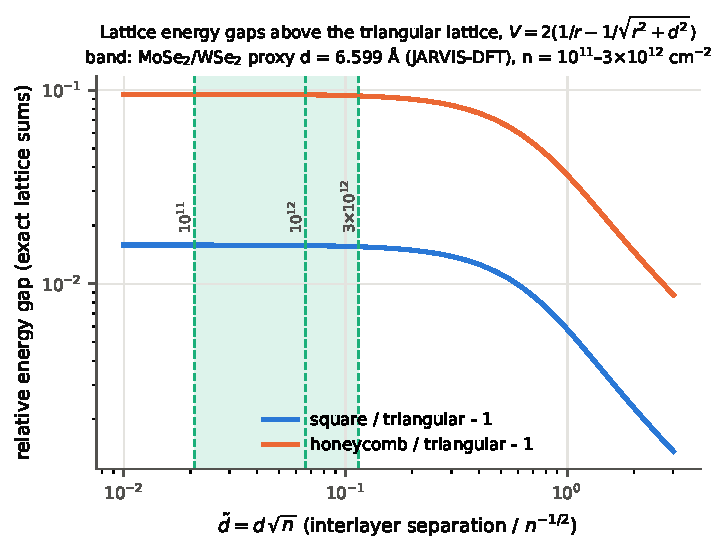
\includegraphics[width=0.49\textwidth]{data/fig_lattice_gaps.pdf}\hfill
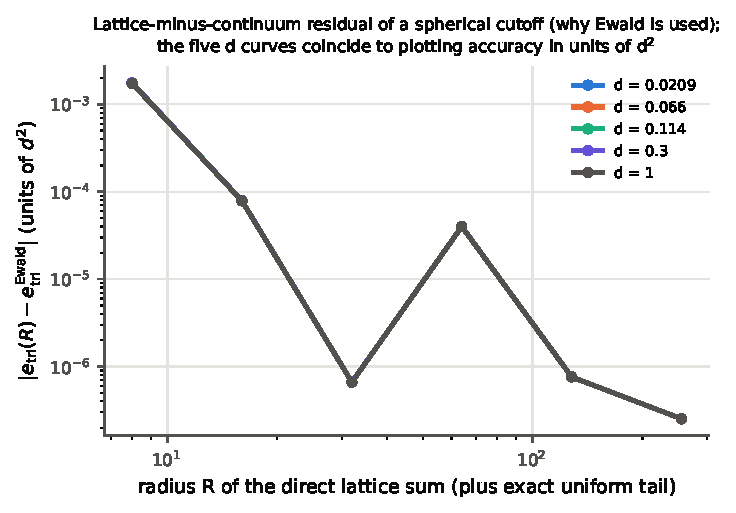
\includegraphics[width=0.49\textwidth]{data/fig_truncation_residual.pdf}
\caption{Left: exact square and honeycomb gaps relative to triangular against $\dt$ \tier{X, DX-X-0002}. Right: residual
of truncated sums with exact tail against $R$ \tier{X, DX-X-0005}. Generated by \texttt{scripts/dipolar\_figures.py}.}
\label{fig:gaps}\label{fig:trunc}
\end{figure}

\paragraph{Lattice gaps \tier{X, DX-X-0002}.} Table~\ref{tab:lat}. On the \DXGridN-point grid
$\dt\in[\DXGridDmin,\DXGridDmax]$, $e_\mathrm{sq}/e_\mathrm{tri}-1$ falls from $\DXSqRelLo$ to $\DXSqRelHi$ and the
honeycomb gap from $\DXHcRelLo$ to $\DXHcRelHi$; both stay positive. In the physical window the gaps are essentially the
pure-dipolar values. These compare two lattices only.

\paragraph{Controls of the relaxation pipeline \tier{X, DX-X-0003}.} At all five $\dt$ (0.0209, 0.066, 0.114, 0.3, 1):
the perfect and the noisy triangular lattices relax back (\DXNPos{} positive controls, $|\text{rel.\ gap}|\le\DXMaxAbsPos$,
0 defects, 0 negative Hessian modes). \emph{Negative controls:} the square lattice is a saddle of the dynamics potential
(\DXSqNegMin--\DXSqNegMax{} negative Hessian modes) and square+noise relaxes to a distorted state still above
triangular (rel.\ gap $\DXSqNoiseMin$--$\DXSqNoiseMax$); two incommensurate boxes stay defected.

\paragraph{Main study, preregistered P1 \tier{X, DX-X-0004}.} \DXNComp{} relaxed competitors: \DXNQuench{} random-start
$T=0$ quenches (at $\dt=0.0209$, $0.066$, $1$), \DXNAnneal{} anneals and \DXNIncomm{} incommensurate boxes (at
$\dt=0.066$), and \DXNSqNoise{} square+noise relaxations. Only the \DXNOpen{} quenches and anneals are open searches;
the \DXNIncomm{} incommensurate boxes and \DXNSqNoise{} square+noise runs (\DXNDesignedNeg{} in all) are designed
negative controls that are expected to sit above triangular. \DXNUndercut{} lie below the exact triangular energy by more
than $10^{-9}$ relative. The most negative competitor gap is $\DXMinRelComp$ (rounding at the perfect lattice;
$\DXMinRelAll$ including the positive controls); the smallest gap among the \DXNAbove{} states not at the lattice is
$\DXMinAbove$. \DXQuenchLattice{} of \DXNQuench{} quenches and \DXAnnealLattice{} of \DXNAnneal{} anneals reach the
perfect lattice; \DXQuenchDefected{} quenches end defected. Truncated and exact gaps differ by $\le\DXMaxSfDiff$.
Caveats: seeds are reused across $\dt$, so the three lattice-reaching quenches share one start (seed 501); only
$\dt=0.066$ received the full preregistered run set; $\dt=0.114$ and $0.3$ have controls only; two zero-defect states sit
above the lattice (probably strained crystallites, not analysed); two of the runs at $\dt=0.066$, \texttt{anneal\_01} and
\texttt{uniform\_04}, start from different seeds but end in the same state ($e=4.43936745573261$, $\psi_6=0.998112$),
so there are fewer independent outcomes than runs. The first attempts at $\dt=0.0209$ and $\dt=1$ (4 quenches, 1 anneal
and 2 incommensurate boxes each, one thread) were killed after about 34~min because they could not finish within the
budget; the driver then kept finished jobs only in memory, so none of their results was ever printed, and those two
$\dt$ were rerun with 2 quenches each using the patched driver (commit \texttt{916fc88}) that prints every result.
Table~\ref{tab:runs}, Figure~\ref{fig:rel}.

\begin{table}[t]\centering\scriptsize
\caption{Relaxed competitors (exact relative gap to the triangular lattice; Hessian of the dynamics potential, -- = not
computed) \tier{X, DX-X-0003, DX-X-0004}.}\label{tab:runs}
\begin{tabular}{rllrrr}\toprule
$\dt$ & run & family & rel.\ gap & defects & neg.\ modes\\\midrule
\tabinput{gen/table_runs.tex}\bottomrule\end{tabular}
\end{table}

\begin{figure}[t]\centering
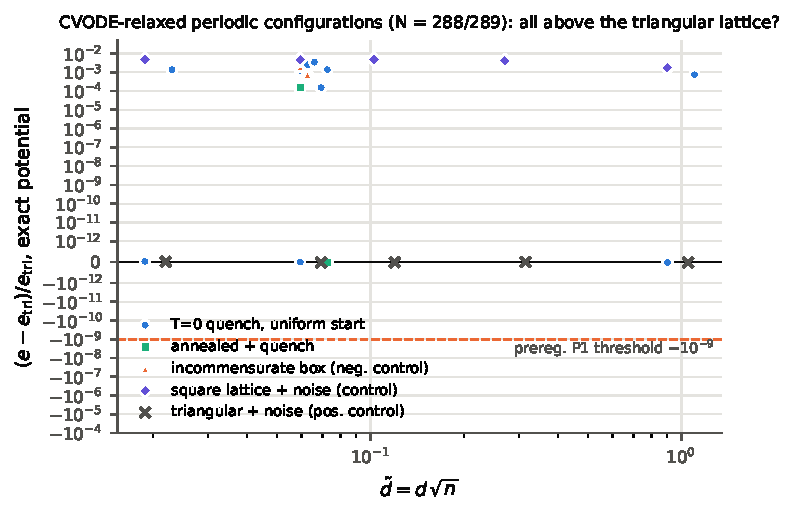
\includegraphics[width=0.7\textwidth]{data/fig_relaxed_gaps.pdf}
\caption{Exact relative gaps of relaxed states \tier{X, DX-X-0004}. Generated by \texttt{scripts/dipolar\_figures.py}.}
\label{fig:rel}
\end{figure}

\section{HuggingFace dataset illustration}\label{sec:hf}
\paragraph{Search.} 26 queries of the Hub (\texttt{HfApi().list\_datasets(search=...)}: C2DB, BiDB, bilayer,
heterobilayer, JARVIS, TMD, MoS2, WSe2, interlayer, \dots) found no dataset of TMD heterobilayers or of interlayer
separations \tier{X, DX-X-0006}.

\paragraph{Dataset used.} \url{colabfit/JARVIS_DFT_3D_12_12_2022}, revision\\
\texttt{f4de0085edcf92885870c67459363d2c7080c90b}, file \texttt{co/co\_0.parquet} (54{,}027{,}813 bytes), a ColabFit
mirror of JARVIS-DFT~\cite{jarvis,colabfit}. The card license is ``unknown'' \tier{L, DX-L-0004}; only derived numbers are
reproduced here, and the upstream figshare license was not checked. JARVIS-DFT uses the vdW-DF-OptB88 functional, which
its authors report gives accurate lattice parameters for van der Waals materials~\cite{jarvis} \tier{L, DX-L-0003}.

\paragraph{What it shows \tier{X, DX-X-0006}.} A selection rule fixed before seeing the output (semiconducting rows, at
least two MX$_2$ layers, metal-plane spacings 4.5--8~\AA, vacuum gaps excluded) gives the adjacent metal-plane spacings of
Table~\ref{tab:hf}. The MoSe$_2$/WSe$_2$ proxy $d=\tfrac12(\DXDMoSe+\DXDWSe)=\DXDproxyA$~\AA{} gives
$\dt=\DXDtElev,\ \DXDtTwelve,\ \DXDtThreeTwelve$ at $n=10^{11},10^{12},3\times10^{12}$~cm$^{-2}$, the density window
of~\cite{wang}. The unscreened square-minus-triangular gap per exciton is then $\DXmeVElev$, $\DXmeVTwelve$ and
$\DXmeVThreeTwelve$~meV (divide by $\varepsilon_r$) \tier{X, DX-X-0007}, about 1.5 to 5 orders of magnitude below the
moir\'e depths of 10s--100~meV. These values multiply the physical $\dt^2$ by the gap $e_\mathrm{sq}-e_\mathrm{tri}$
evaluated at the nearest simulated $\dt$ (0.0209, 0.066, 0.114), not at the physical $\dt$ (0.02087, 0.06599, 0.1143);
evaluating the gap at $\dt=0.1143$, the stage-4 auditor gets 0.224~meV at $3\times10^{12}$~cm$^{-2}$, a 0.5\% difference.

\begin{table}[t]\centering\small
\caption{Adjacent metal-plane spacings from the HuggingFace JARVIS-DFT mirror (ColabFit names) \tier{X, DX-X-0006}.}\label{tab:hf}
\begin{tabular}{lp{6.4cm}rrr}\toprule
material & rows & spacings & mean (\AA) & range (\AA)\\\midrule
\tabinput{gen/table_hf.tex}\bottomrule\end{tabular}
\end{table}

\paragraph{Caveats.} No heterobilayer row exists on the Hub, so the proxy comes from homo-stacks; the metal-plane spacing
is used as the electron--hole separation, which is an assumption \tier{C, DX-C-0005}; the MoS$_2$ row is a bulk-like cell,
not a slab; no WS$_2$ row passed the selection. The dataset illustrates the physical $\dt$ range; it does not test the
theorem.

\section{Claim ledger}\label{sec:ledger}
\texttt{ledger/build\_ledger.py} files \DXLedgerN{} claims: \DXLedgerA{} at Tier~A, \DXLedgerL{} at L, \DXLedgerC{} at C and
\DXLedgerX{} at X. Each has a content-addressed evidence blob in \texttt{ledger/evidence/}: verbatim axiom lines and source
hashes (A), verbatim excerpts in \texttt{ledger/sources/excerpts.json} (L), argument text (C), and result files with
\texttt{claim\_licence: false} (X). The Elenchus gate (\texttt{tools/ledger.py ledger.json -{}-evidence-dir evidence},
output in \texttt{ledger/gate\_output.txt}) exits with code~\DXGateExit. It reports \textbf{\DXGateBlock{} blocking findings}
and \textbf{\DXGateFlag{} flags}, all \texttt{LEDGER\_UNAUDITED\_TIER\_A}: no person has certified that the Tier~A
statements mean what their glosses say. The flags remain open. The L excerpts are prose, not theorem statements, so the
Elenchus citation gate (\texttt{citation\_check.py}, theorem/lemma excerpts only) was not run on them.

\section{Limitations}\label{sec:lim}
\begin{itemize}
\item \textbf{Upstream dependence.} Every triangular-lattice statement rests on openai/math's
\lean{universal\_energy\_minimum} (AI-generated, not peer reviewed; the human-literature conjecture was stated open in
2019~\cite{ps}) and on the
fidelity of its definitions (\lean{energy}, \lean{LocallyFinite}, \lean{DensityOne}, D2's \lean{DensityRho}).
\item \textbf{Verification status.} The prior-round module was re-checked by an AI verifier and the Multipolar module
was re-elaborated from source by a separate AI auditor; neither by a person. The Step-1 module added in this revision
is producer-checked only. The paper-stage reruns (Section~\ref{sec:repro}) come from the same AI pipeline as the
producer. The auditor did not re-run the crate tests (its isolation guard refused \texttt{cargo} on this worktree).
\item \textbf{Novelty is small.} Complete monotonicity of $g_d$ is elementary (Bernstein); the corollary is immediate
given upstream. A literature search found no explicit statement, which is weak evidence \tier{C, DX-C-0003}.
\item \textbf{Model.} Classical, rigid, unscreened point dipoles, no quantum kinetic energy, no moir\'e potential; real
excitons in the physical window are a quantum gas.
\item \textbf{Numerics.} \DXNComp{} competitors from one box shape and $N$, of which only \DXNOpen{} are open searches
and two share a final state; reduced run counts versus the preregistration; reused seeds; Ewald energies instead of the
preregistered truncated sum. Tier~X never supports the theorem.
\item \textbf{Data.} Homo-stack proxy for a heterobilayer quantity; license ``unknown'' on the dataset card.
\end{itemize}

\section{Reproducibility}\label{sec:repro}
AutoevolveAI files are uncommitted on top of base \texttt{db794dd98d12c2a79702eab5651ae7c36a35ea27} (branch
\texttt{worktree-openai-math-discovery}). Lean source sha256 values (they \DXShaMatch{} those recorded at stage~1):
\begin{itemize}\scriptsize
\item \texttt{DipolarExciton.lean}: \texttt{\DXShaPrior}
\item \texttt{DipolarExcitonMultipolar.lean}: \texttt{\DXShaMulti}
\item \texttt{DipolarExcitonMultipolarControls.lean}: \texttt{\DXShaCtl}
\item \texttt{Triangular/AnyDensity.lean}: \texttt{\DXShaAnyD}
\item \texttt{DipolarExcitonStep1.lean}: \texttt{\DXShaStepOne}
\item \texttt{DipolarExcitonStep1Controls.lean}: \texttt{\DXShaStepOneCtl}
\end{itemize}
(the last two, added in this revision, \DXShaStepOneMatch{} the values recorded when they were compiled).
rusty-SUNDIALS commits on branch \texttt{physics/ar-dipolar-exciton-2026-10-25} (not pushed):
\begin{itemize}\small
\item preregistration \texttt{4feb027eb502ff0936a28f8168499b6fef25e276};
\item code \texttt{17ea6beccd044a02f46a8d8f7f04c76f31ee33f0};
\item per-job output patch \texttt{916fc88c8cebab15426427a5601a38278a1467c2};
\item results \texttt{272a09e62c1b9b36eabc167cdafaa2845fbe9198}.
\end{itemize}
The $\dt=0.066$ main run and the controls used the binary built from \texttt{17ea6be} (before \texttt{cargo fmt}, a
formatting-only change).
\begin{lstlisting}[basicstyle=\ttfamily\scriptsize]
taskset -c 4-7 python3 scripts/certified_numerics/lean_pinned.py compile formal_cert/Autoresearch/DipolarExcitonMultipolar.lean \
  --olean Autoresearch.DipolarExcitonMultipolar --json-out results/autoresearch/2026-10-25/H1/contribution/compile_attempt1.json
taskset -c 4-7 python3 scripts/certified_numerics/lean_pinned.py compile formal_cert/Autoresearch/DipolarExcitonMultipolarControls.lean \
  --json-out results/autoresearch/2026-10-25/H1/contribution/compile_controls.json
taskset -c 4-7 python3 scripts/certified_numerics/lean_pinned.py compile formal_cert/Autoresearch/DipolarExcitonStep1.lean \
  --olean Autoresearch.DipolarExcitonStep1 --json-out results/autoresearch/2026-10-25/H1/contribution/compile_step1.json
taskset -c 4-7 python3 scripts/certified_numerics/lean_pinned.py compile formal_cert/Autoresearch/DipolarExcitonStep1Controls.lean \
  --json-out results/autoresearch/2026-10-25/H1/contribution/compile_step1_controls.json
CARGO_TARGET_DIR=... cargo test --release -j 2 --offline --manifest-path <rusty-wt>/Cargo.toml -p qf-yukawa-crystal -- --test-threads=2
dipolar_crystal refs|gaps|controls <crate>;  dipolar_crystal main <crate> 0.066 8 2
DIPOLAR_THREADS=1 dipolar_crystal main <crate> 0.0209 2 0 0;  DIPOLAR_THREADS=1 dipolar_crystal main <crate> 1 2 0 0
python -I scripts/dipolar_hf_download.py <hf-data>/dipolar_exciton colabfit/JARVIS_DFT_3D_12_12_2022@f4de0085...:co/co_0.parquet ...
python -I scripts/dipolar_tmd_extract.py ... ; python -I scripts/dipolar_physical_d.py ...
python -I scripts/dipolar_independent_check.py ... ; python -I scripts/dipolar_figures.py ...
python -I papers/ar_dipolar_exciton/ledger/build_ledger.py ; python -I papers/ar_dipolar_exciton/ledger/run_gate.py
python -I papers/ar_dipolar_exciton/gen_inputs.py ; pdflatex main.tex (twice)
\end{lstlisting}
\emph{Paper-stage reruns} (\tier{X, DX-X-0008}), by the same AI pipeline, not by a person: crate tests
\DXTestsPassed{} passed, \DXTestsFailed{} failed, \DXTestsIgnored{} ignored (the ignored test predates this work); Lean
recompile of the controls file (imports the stage-1 oleans, so it re-reads axioms rather than re-elaborating the module):
\DXRecompileCtl; Lean recompile of the Multipolar source without writing oleans (re-elaborates the new module against the prior-round
olean): \DXRecompileSrc. Neither rerun separates producer from verifier.

\begin{thebibliography}{99}\small
\bibitem{oai} OpenAI, \emph{Universal optimality of the triangular lattice}, OpenAI Math release, github.com/openai/math,
commit \texttt{fd4aeeb2ee4fc729c18d98444fed42fd0529eeeb} (2026). AI-generated; not peer reviewed.
\bibitem{ps} M.~Petrache, S.~Serfaty, \emph{Crystallization for Coulomb and Riesz interactions as a consequence of the
Cohn--Kumar conjecture}, arXiv:1908.09714v3 (2019).
\bibitem{wang} J.~Wang, Q.~Shi, E.-M. Shih, L.~Zhou, W.~Wu, Y.~Bai, D.~A. Rhodes, K.~Barmak, J.~Hone, C.~R. Dean,
X.-Y. Zhu, \emph{Diffusivity reveals three distinct phases of interlayer excitons in MoSe$_2$/WSe$_2$ heterobilayers},
arXiv:2001.03812v5.
\bibitem{jarvis} K.~Choudhary et al., \emph{The Joint Automated Repository for Various Integrated Simulations (JARVIS) for
data-driven materials design}, arXiv:2007.01831v2; publication doi:10.1038/s41524-020-00440-1 as given in the dataset
card (journal volume and page not verified by us).
\bibitem{colabfit} K.~Choudhary et al., \emph{JARVIS DFT 3D 12 12 2022}, ColabFit (2023), doi:10.60732/e9e65ccd;
HuggingFace \texttt{colabfit/JARVIS\_DFT\_3D\_12\_12\_2022}, revision \texttt{f4de0085edcf92885870c67459363d2c7080c90b}.
\bibitem{d2} X.~Callens, \emph{Riesz-energy, finiteness and every-density corollaries of the openai/math planar
universal-optimality theorem, kernel-checked in Lean 4}, doi:10.5281/zenodo.23285631 (2026); D2 is its every-density
module \texttt{formal\_cert/Triangular/AnyDensity.lean}.
\bibitem{uot} X.~Callens, \emph{Planar universal optimality, tiered: kernel-checked consequences, a non-uniqueness
theorem, and a CVODE N-body consistency check for the Yukawa interaction}, preprint v2, doi:10.5281/zenodo.23293429 (2026).
\bibitem{txt} X.~Callens, \emph{The Triangular Lattice and Universal Optimality} (textbook), doi:10.5281/zenodo.23295142 (2026).
\end{thebibliography}
\noindent This preprint applies the approach of~\cite{uot,txt} (kernel-checked consequences of upstream for explicit
interactions) to the bilayer dipolar-exciton interaction.
\end{document}
